\subsection{Definizione di una Politica Temporale di Ricalcolo}\label{policy}

L'utente, al di là delle varie impostazioni di collegamento della rete bayesiana caricata al flusso dati, deve inoltre avere la possibilità di definire una Politica Temporale per il ricalcolo delle probabilità associate ai nodi delle rete in fase di monitoraggio.\\
Per poter effettuare questa operazione l'utente deve, come prima cosa, accedere al pannello per la definizione della politica temporale tramite il pulsante \textbf{Imposta} posizionato accanto alla label "Imposta politica temporale" (Figura \ref{Pannello}).\\
~\\
L'utente deve quindi configurare la politica temporale attraverso la compilazione dei tre campi dati: "Secondi", "Minuti" ed "Ore" presenti in Figura \ref{PannelloPolicy}. Attraverso questi campi è possibile deinire con precisione e semplicità la politica temporale, ovvero il temout ciclico per il ricalcolo delle probabilità in fase di monitoraggio.

\begin{figure}[H]
	\begin{center}
		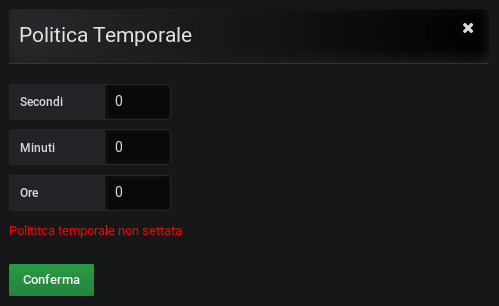
\includegraphics[scale=0.6]{./images/PannelloPolicy.png}
		 \caption{Pannello di configurazione della Politica Temporale}	
		 \label{PannelloPolicy}
	\end{center}
\end{figure} 

L'utente deve infine confermare le proprie scelte attraverso il pulsante \textbf{Conferma}, presente anch'esso in Figura \ref{PannelloPolicy}.
~\\
A seguito della corretta definizione della politica temporale, l'utente verrà avvisato del buon esito dell'operazione da un messaggio di notifica (Figura \ref{NotificaPolicy}). 

\begin{figure}[H]
	\begin{center}
		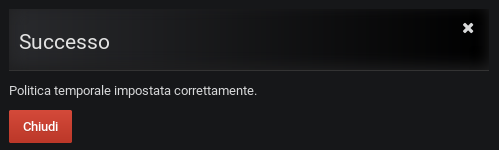
\includegraphics[scale=0.6]{./images/NotificaPolicy.png}
		 \caption{Notifica avvenuto Settaggio della Politica Temporale}	
		 \label{NotificaPolicy}
	\end{center}
\end{figure}

~\\
\textbf{\textcolor{red}{ATTENZIONE}}: Nel caso in cui l'utente abbia commesso degli errori in fase di compilazione dei campi dati, l'operazione non va a buon fine e l'utente viene avvisato degli errori commessi da un messaggio di errore (Figura \ref{ErrorePolicy}). Nello specifico i campi dati \textbf{"Secondi"} e \textbf{"Minuti"} accettano numeri interi compresi tra 0 e 59, mentre il campo \textbf{"Ore"} deve essere compilato con numeri interi positivi.

\begin{figure}[H]
	\begin{center}
		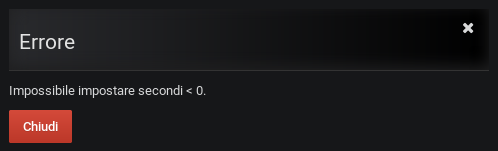
\includegraphics[scale=0.6]{./images/ErrorePolicy.png}
		 \caption{Messaggio di Errore configurazione Politica Temporale}	
		 \label{ErrorePolicy}
	\end{center}
\end{figure}

